\documentclass[10pt, a4paper]{article} %Definerer skriftstørrelse, arktrype( eks a0paper, ..., a6paper, letterpaper....), dokumenttype(article, report, book, letter, beamer(presentasjon).   
\usepackage[font=small, labelfont=bf]{caption}
\usepackage{graphicx}
\usepackage{amsmath, amssymb} %  matematiske funskjoner og symboler. 
\usepackage{listings}
\usepackage{url} % urls in the bibliograpy
\usepackage[utf8]{inputenc} % 
\usepackage{float}  %
\usepackage{subcaption} % NOT compatible with the subfig package
\usepackage{authblk}
\usepackage{siunitx}



\usepackage[ 
total={250mm,297mm},  
left=25mm,
 right=25mm,
 top=10mm,
 bottom=20mm]{geometry} % kan endre på marger 
%%%%%%%%%%%%%%%%%%%%%%%%%%%%%%%%%%%%%%%%%%%%%%%%%%%%%%%%%%%%%%%%
% Gode infosider:
% https://no.sharelatex.com/learn/Creating_a_document_in_LaTeX 
% https://no.sharelatex.com/learn/Page_size_and_margins
 
%%%%%%%%%%%%%%%%%%%%%%%%%%%%%%%%%%%%%%%%%%%%%%%%%%%%%%%%%%%%%%%%
% Det som inkluderes i \maketitle
\title{Report project superpercomuters}
\author[]{Jon Christian Halvorsen, Monica Kappelslåen Plassen, Anette Fossum Morken}
\date{}
%%%%%%%%%%%%%%%%%%%%%%%%%%%%%%%%%%%%%%%%%%%%%%%%%%%%%%%%%%%%%%%
\begin{document}
\maketitle

%\begin{abstract}

%\end{abstract}

\section*{Theory}
In this project we are studying the two-dimensional Poisson problem
\begin{align}
-\nabla^2u&=f \quad\quad\text{ in } \Omega=(0,1)\times(0,1)\\
u&=0 \quad\quad\text{ on } \partial \Omega, \nonumber
\label{Poisson}
\end{align}
where $f$ is given load function and $u$ is the solution. We have been using two different load functions
\begin{align*}
f(x,y)&=1
\end{align*}
and
\begin{align}
f(x,y)&=5\pi^2\sin(2\pi x)\sin(\pi y) \quad\text{with exact solution} \\
u(x,y)&=\sin(2\pi x)\sin(\pi y).\nonumber
\label{loadfunc2}
\end{align}
We discretize the Laplace operator with the five-point stencil and use regular finite difference grid with $(n+1)$ points in each direction and use a local numbering scheme. This results in a SPD algebraic system
\begin{equation}
	\mathbf{AU} = \mathbf{B}.
	\label{system1}
\end{equation}
Since the matrix $\mathbf{A}$ resulted from applying the three point formula in $x$ and $y$, it is a tensor product operator. Thus \eqref{system1} can be stated as 
\begin{equation}
	\mathbf{TU} + \mathbf{UT} = \mathbf{B}
\end{equation}
where $\mathbf{T}$ (skrive noe om T, begrunne at den er SPD...). Since $\mathbf{T}$ is SPD, we know we can perform an eigendecomposition $\mathbf{T} = \mathbf{Q\Lambda Q^T}$. Now, letting $\mathbf{\widetilde{B}} = \mathbf{Q^TBQ^T}$ and $\mathbf{\widetilde{U}} = \mathbf{Q^TUQ}$, we finally arrive at the system 
\begin{equation}
	\mathbf{\Lambda\widetilde{U}} + \mathbf{\widetilde{U}\Lambda} = \mathbf{\widetilde{B}}.
	\label{system2}
\end{equation}
Finding $\mathbf{\widetilde{U}}$ from \eqref{system2} is a simple calculation, and we can from this get the final answer $\mathbf{U}$. Now we utilize what we know about the Poisson problem to avoid the two matrix-matrix products needed to compute both $\mathbf{\widetilde{B}}$ and $\mathbf{U}$, which is done in $\mathcal{O}(N^3)$ time. \\
\\
(Forklare hvorfor vi kan bruke DST)
\\
\\
Let $\mathbf{S}$ denote the discrete sine transform, and $\mathbf{S}^{-1}$ be the inverse transform. We can now express $\mathbf{Q} = \sqrt{\frac{N}{2}\mathbf{S}}$ and $\mathbf{Q}^T = \sqrt{\frac{2}{N}}\mathbf{S}^{-1}$, and therefore $\mathbf{\widetilde{B}} = \mathbf{S}^{-1}((\mathbf{SB})^T)$ and $\mathbf{U} = \mathbf{S}^{-1}(\mathbf{S}(\mathbf{\widetilde{U}}^T))^T$. Both of these operations can be done in $\mathcal{O}((N^2\log{N})$ time. 

\section*{Our code}
We solved this problem with our program. The pseudocode to our program is shown i figure ..... 



\section*{Results}

\begin{figure}[h]
\centering
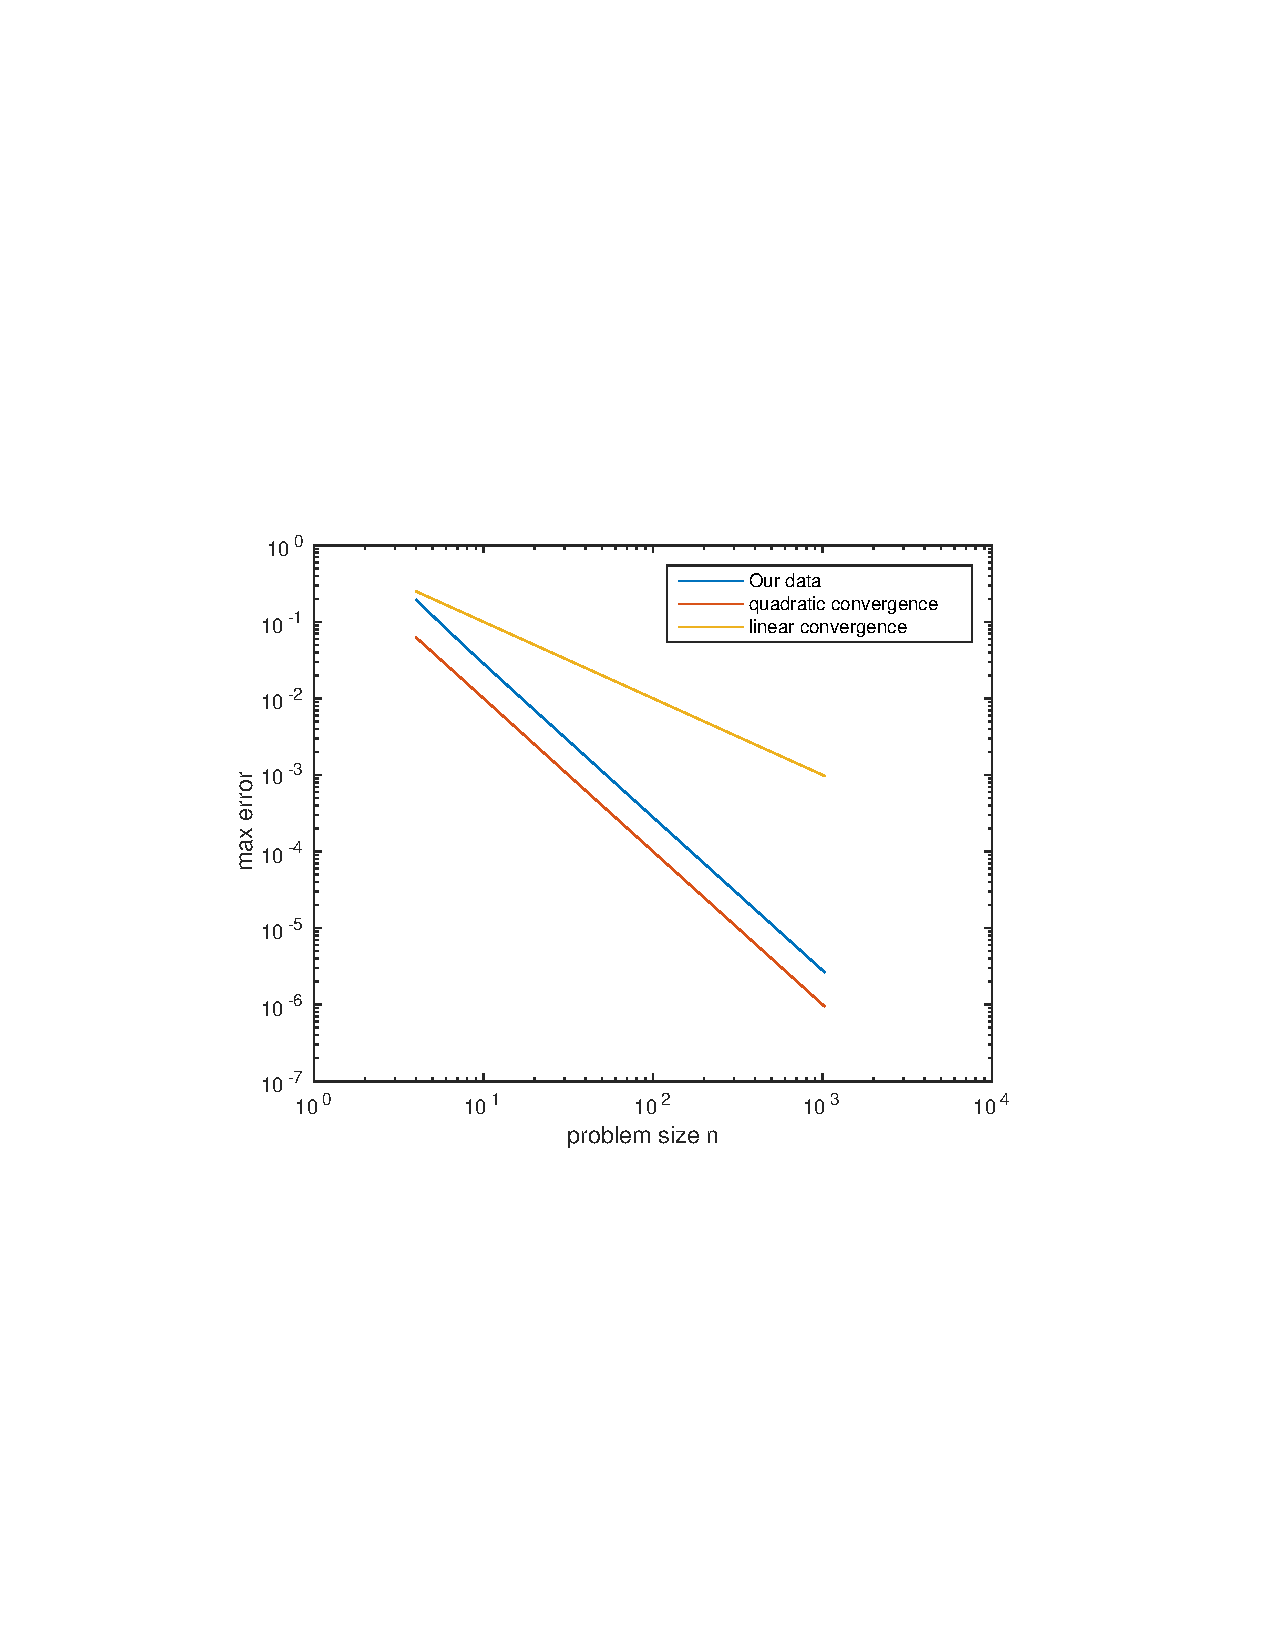
\includegraphics[width=0.7\linewidth, trim= 3cm 8.5cm 3cm 9cm, clip=true]{checkConv}
\caption{Shows that the result from the convergence test compared with curves with slope $h$ and $h^2$}
\label{fig:checkConv}
\end{figure}

%%%%%%%%%%%%%%%%%%%%%%%%%%%%%%%%%%%%%%%%%%%%%%%%%%%%%%%%%
% REFERANSER
%\nocite{*} %gjør at alle kilder vises ikke bare de det refereres til.
%\addcontentsline{toc}{section}{Kilder} % Setter kilder inn i innholdsfortegnelsen
%\renewcommand{\refname}{Kilder} % Endrer overkriften fra References til Kilder
%\bibliographystyle{plain}
%\bibliography{mal_Latex}
\end{document}
